\documentclass[12pt,a4paper]{article}

% ── Encoding & language ──
\usepackage[utf8]{inputenc}
\usepackage[T1]{fontenc}
\usepackage[brazil]{babel}

% ── Layout ──
\usepackage[margin=2.5cm]{geometry}
\usepackage{setspace}\onehalfspacing

% ── Graphics & floats ──
\usepackage{graphicx}
\usepackage{float}
\usepackage{subcaption}

% ── Math ──
\usepackage{amsmath,amssymb}

% ── Code listings ──
\usepackage{listings}
\usepackage{xcolor}
\lstset{
  language=Python,
  basicstyle=\ttfamily\footnotesize,
  keywordstyle=\color{blue}\bfseries,
  stringstyle=\color{red!70!black},
  commentstyle=\color{green!50!black}\itshape,
  numbers=left,
  numberstyle=\tiny\color{gray},
  numbersep=6pt,
  breaklines=true,
  frame=single,
  backgroundcolor=\color{gray!5},
  tabsize=4,
  showstringspaces=false,
}

% ── Hyperlinks ──
\usepackage{hyperref}
\hypersetup{colorlinks=true,linkcolor=blue,citecolor=blue,urlcolor=blue}

% ══════════════════════════════════════════════════════════════════════════
\begin{document}

% ── COVER ─────────────────────────────────────────────────────────────────
\begin{titlepage}
\centering
\vspace*{1cm}

{\large MINISTÉRIO DA DEFESA\\
DEPARTAMENTO DE CIÊNCIA E TECNOLOGIA\\
INSTITUTO MILITAR DE ENGENHARIA\\[4pt]
\textit{(Real Academia de Artilharia, Fortificação e Desenho, 1792)}}

\vspace{1.5cm}
{\Large\bfseries ENGENHARIA DA COMPUTAÇÃO}

\vspace{0.5cm}
{\Large COMPUTAÇÃO GRÁFICA}

\vspace{0.5cm}
{\large PROFESSOR: CORONEL MADEIRA}

\vspace{3cm}
{\LARGE\bfseries Image Stitching --- Geração de Panoramas}

\vspace{3cm}
{\Large
João Victor Paim\\[6pt]
Gabriel Dias Vilela}

\vfill
{\large RIO DE JANEIRO\\2026}
\end{titlepage}

% ── TABLE OF CONTENTS ─────────────────────────────────────────────────────
\newpage
\tableofcontents
\newpage

% ══════════════════════════════════════════════════════════════════════════
\section{Introdução}

O presente trabalho descreve a implementação de um sistema de \textit{Image Stitching}
para a geração de fotografias panorâmicas, desenvolvido no contexto da disciplina de
Computação Gráfica. A composição de panoramas é um problema clássico de visão
computacional que envolve a combinação de múltiplas imagens de uma mesma cena,
capturadas sob diferentes pontos de vista, em uma única imagem composta e
visualmente contínua.

O desafio central reside no fato de que duas fotografias de um mesmo cenário, tiradas
de posições ligeiramente diferentes, relacionam-se por uma \textbf{transformação
projetiva (homografia)}. Para estimar essa transformação e compor o panorama, o
pipeline implementado neste trabalho é composto por quatro etapas fundamentais:

\begin{enumerate}
  \item \textbf{Seleção manual de pontos correspondentes} --- o usuário identifica 4
        pares de pontos em comum entre as duas imagens;
  \item \textbf{Cálculo da homografia via DLT} --- a matriz $3\times3$ é estimada
        resolvendo o sistema $A\mathbf{h}=\mathbf{0}$ por SVD;
  \item \textbf{Transformação da imagem (warping manual)} --- cada pixel de saída é
        mapeado de volta à imagem de origem pela homografia inversa;
  \item \textbf{Composição (stitching) e fusão} --- as imagens transformada e de
        referência são coladas em um canvas comum, com blend ponderado por distância.
\end{enumerate}

A implementação foi realizada em Python, utilizando NumPy para álgebra linear e
Matplotlib para visualização. A seleção dos pontos correspondentes é feita por meio
de um script auxiliar com interface gráfica.

Dois exemplos de teste foram utilizados, e os resultados para ambos são apresentados
nas seções seguintes.

% ══════════════════════════════════════════════════════════════════════════
\section{Fundamentação Teórica}

\subsection{Coordenadas Homogêneas}

Em geometria projetiva, um ponto $\mathbf{p}=(x,y)$ no plano euclidiano é
representado em coordenadas homogêneas como
$\tilde{\mathbf{p}}=(x,\;y,\;1)^T$.
Qualquer vetor $(\lambda x,\;\lambda y,\;\lambda)^T$ com $\lambda\neq0$ representa o
mesmo ponto. A conversão de volta é:
\begin{equation}
(x,y)=\left(\frac{\tilde{x}}{\tilde{w}},\;\frac{\tilde{y}}{\tilde{w}}\right)
\end{equation}

\subsection{Definição da Homografia}

Uma homografia $H$ é uma transformação projetiva $\mathbb{P}^2\to\mathbb{P}^2$ que
mapeia pontos entre dois planos:
\begin{equation}
\tilde{\mathbf{p}}' \sim H\,\tilde{\mathbf{p}},\qquad
H = \begin{bmatrix}
  h_{11} & h_{12} & h_{13}\\
  h_{21} & h_{22} & h_{23}\\
  h_{31} & h_{32} & h_{33}
\end{bmatrix}
\end{equation}
Como $H$ é definida a menos de escala, possui \textbf{8 graus de liberdade}. Cada par
de pontos correspondentes fornece 2 equações, logo são necessários no mínimo
\textbf{4 pares} para determinar $H$.

\subsection{Transformada Linear Direta (DLT)}

Dado um par de correspondências $\mathbf{p}_i=(x_i,y_i)$ e
$\mathbf{p}'_i=(x'_i,y'_i)$, a relação
$\tilde{\mathbf{p}}'_i\times H\tilde{\mathbf{p}}_i=\mathbf{0}$ gera, para cada
par, duas linhas do sistema:
\begin{equation}
\begin{bmatrix}
-x_i & -y_i & -1 & 0 & 0 & 0 & x'_ix_i & x'_iy_i & x'_i\\
 0 & 0 & 0 & x_i & y_i & 1 & -y'_ix_i & -y'_iy_i & -y'_i
\end{bmatrix}
\mathbf{h} = \mathbf{0}
\end{equation}
Empilhando as equações de $N\geq4$ pares, obtém-se $A\mathbf{h}=\mathbf{0}$ com
$A\in\mathbb{R}^{2N\times9}$. A solução de mínimos quadrados é o vetor singular
associado ao menor valor singular de $A$, obtido pela decomposição SVD:
\begin{equation}
\mathbf{h}^* = \arg\min_{\|\mathbf{h}\|=1}\|A\mathbf{h}\|^2 = \mathbf{v}_9
\end{equation}

\subsection{Warping Perspectivo por Mapeamento Inverso}

Para transformar uma imagem pela homografia $H$, empregamos o
\textbf{mapeamento inverso}: para cada pixel $(x',y')$ da imagem de saída, calculamos
a coordenada correspondente na imagem de entrada:
\begin{equation}
\begin{bmatrix}x\\y\\w\end{bmatrix}
= H^{-1}\begin{bmatrix}x'\\y'\\1\end{bmatrix},
\qquad
\text{pixel de entrada} = \left(\frac{x}{w},\;\frac{y}{w}\right)
\end{equation}
A amostragem é feita por vizinho mais próximo (\textit{nearest-neighbour}). Pixels
cuja coordenada de origem cai fora dos limites da imagem recebem valor zero (preto).

A implementação é vetorizada com NumPy, processando todos os pixels do canvas em uma
única operação matricial.

\subsection{Cálculo do Canvas de Saída}

Para determinar as dimensões do panorama, os quatro cantos da imagem a ser
transformada são projetados por $H$:
\begin{equation}
\tilde{\mathbf{c}}'_j = H\,\tilde{\mathbf{c}}_j,\quad j=1,\ldots,4
\end{equation}
A envoltória de todos os cantos (das duas imagens) define o tamanho do canvas. Como
a projeção pode gerar coordenadas negativas, aplica-se uma translação $T$:
\begin{equation}
T = \begin{bmatrix}1&0&-x_{\min}\\0&1&-y_{\min}\\0&0&1\end{bmatrix}
\end{equation}
A homografia composta $T\cdot H$ posiciona corretamente a imagem no canvas.

\subsection{Fusão de Imagens}

Na composição simples, as regiões de sobreposição recebem a \textbf{média aritmética}
dos valores das duas imagens. Para melhorar a transição, implementamos também um
\textit{blend} ponderado pela distância de cada pixel à borda da respectiva região
válida. A máscara de distância é calculada por varreduras horizontais e verticais:
\begin{equation}
R(x,y) = \frac{w_A(x,y)\cdot I_A(x,y) + w_B(x,y)\cdot I_B(x,y)}
               {w_A(x,y) + w_B(x,y) + \varepsilon}
\end{equation}
onde $w_A$ e $w_B$ são as distâncias normalizadas à borda e $\varepsilon=10^{-10}$
evita divisão por zero.

% ══════════════════════════════════════════════════════════════════════════
\section{Detalhamento da Implementação}

A solução foi organizada em um Jupyter Notebook (\texttt{photo\_stitching.ipynb})
acompanhado de um script auxiliar para seleção de pontos
(\texttt{select\_points.py}).

\subsection{Seleção Manual de Pontos (\texttt{select\_points.py})}

O script abre as duas imagens em uma janela Matplotlib interativa. O usuário clica
alternadamente em pontos correspondentes (4 pares), e as coordenadas são salvas em um
arquivo \texttt{points.json}. As cores dos marcadores identificam cada par.

\subsection{Cálculo da Homografia (\texttt{compute\_homography})}

A função recebe dois conjuntos de pontos $N\times2$, monta a matriz
$A\in\mathbb{R}^{2N\times9}$ conforme a formulação DLT e resolve via
\texttt{np.linalg.svd}. O vetor singular associado ao menor valor singular é
reorganizado em uma matriz $3\times3$.

\subsection{Warping Perspectivo (\texttt{warp\_perspective})}

Implementa o mapeamento inverso vetorizado:
\begin{enumerate}
  \item Cria uma grade de coordenadas homogêneas $(x',y',1)$ para todos os pixels de
        saída via \texttt{np.mgrid};
  \item Multiplica pela inversa $M^{-1}$ em uma única operação matricial;
  \item Divide pela coordenada homogênea $w$;
  \item Arredonda para o vizinho mais próximo e copia os pixels válidos.
\end{enumerate}

\subsection{Composição e Stitching}

O canvas é dimensionado pela envoltória dos cantos projetados de ambas as imagens. A
imagem A é transformada para o canvas via \texttt{warp\_perspective}; a imagem B é
colocada diretamente na posição correspondente. Na sobreposição, a média simples é
aplicada.

\subsection{Blend Ponderado por Distância (\texttt{get\_distance\_mask})}

A máscara de pesos é construída por 4 varreduras (esquerda, direita, cima, baixo),
cada uma vetorizada por linha/coluna com \texttt{np.where}. O mínimo das 4 direções
aproxima a distância Chebyshev ($L_\infty$) à borda da região válida. Os pesos são
normalizados para $[0,1]$.

% ══════════════════════════════════════════════════════════════════════════
\section{Análise de Resultados}

\subsection{Exemplo 1}

\subsubsection{Imagens de Entrada}

\begin{figure}[H]
\centering
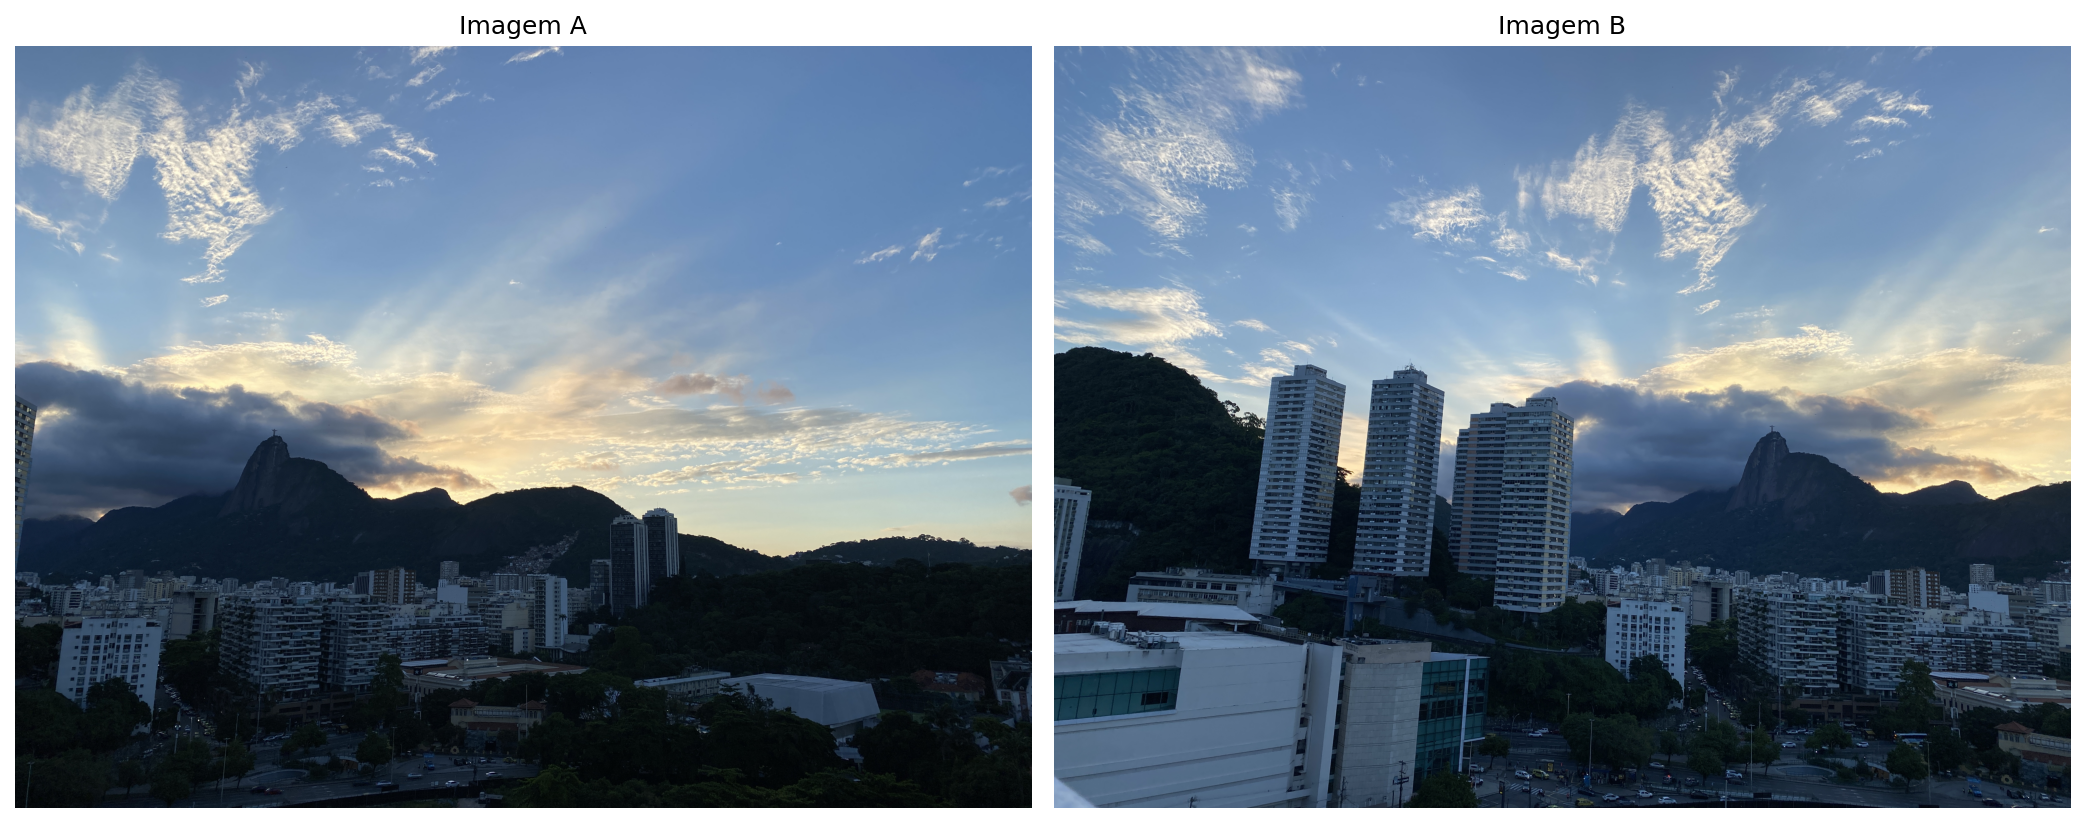
\includegraphics[width=\textwidth]{figures/ex1_inputs.png}
\caption{Imagens de entrada --- Exemplo 1.}
\label{fig:ex1_inputs}
\end{figure}

\subsubsection{Pontos Correspondentes}

\begin{figure}[H]
\centering
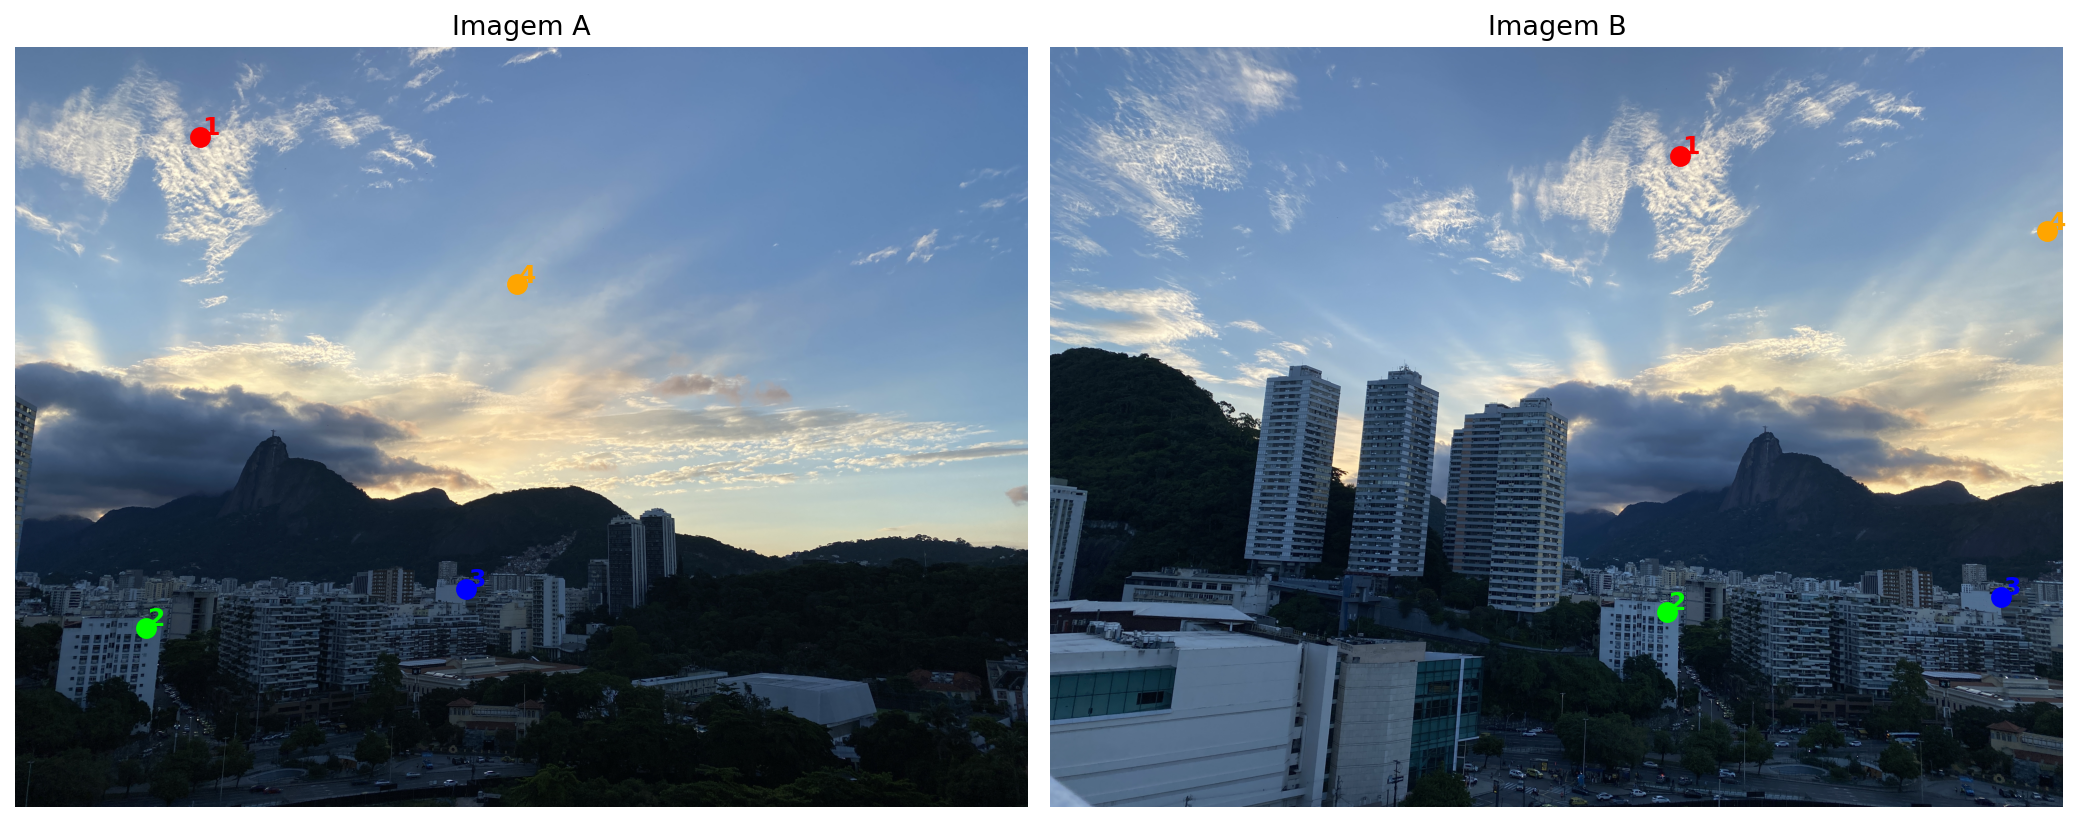
\includegraphics[width=\textwidth]{figures/ex1_points.png}
\caption{Pontos correspondentes selecionados manualmente --- Exemplo 1.}
\label{fig:ex1_points}
\end{figure}

\subsubsection{Imagem Transformada (Warped)}

\begin{figure}[H]
\centering
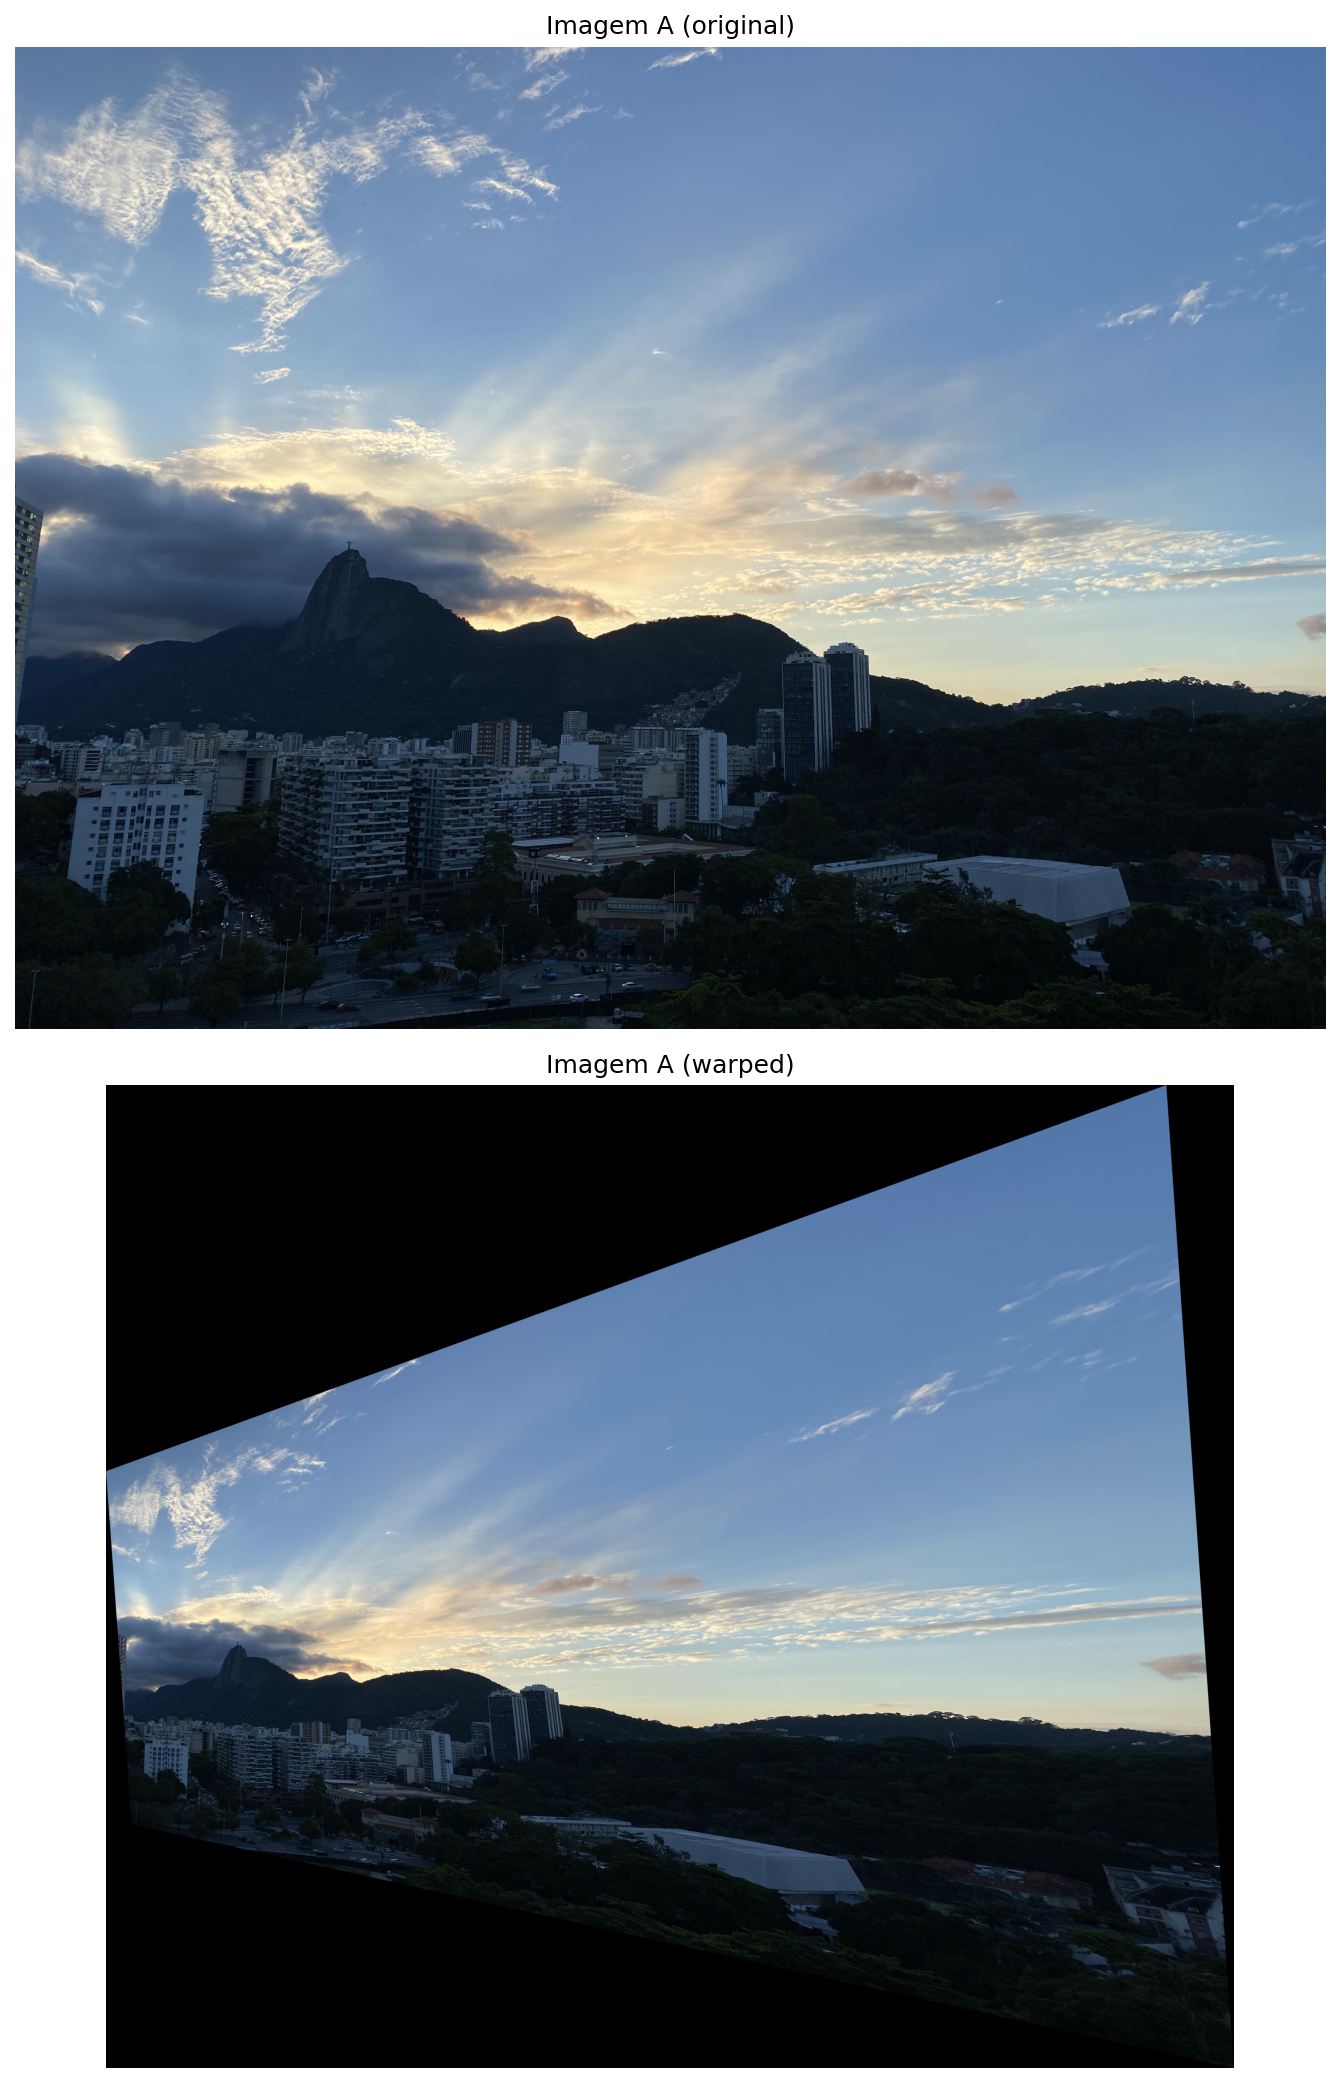
\includegraphics[width=0.85\textwidth]{figures/ex1_warped.png}
\caption{Imagem A original (acima) e após aplicação da homografia (abaixo) --- Exemplo 1.}
\label{fig:ex1_warped}
\end{figure}

\subsubsection{Panorama com Média Simples}

\begin{figure}[H]
\centering
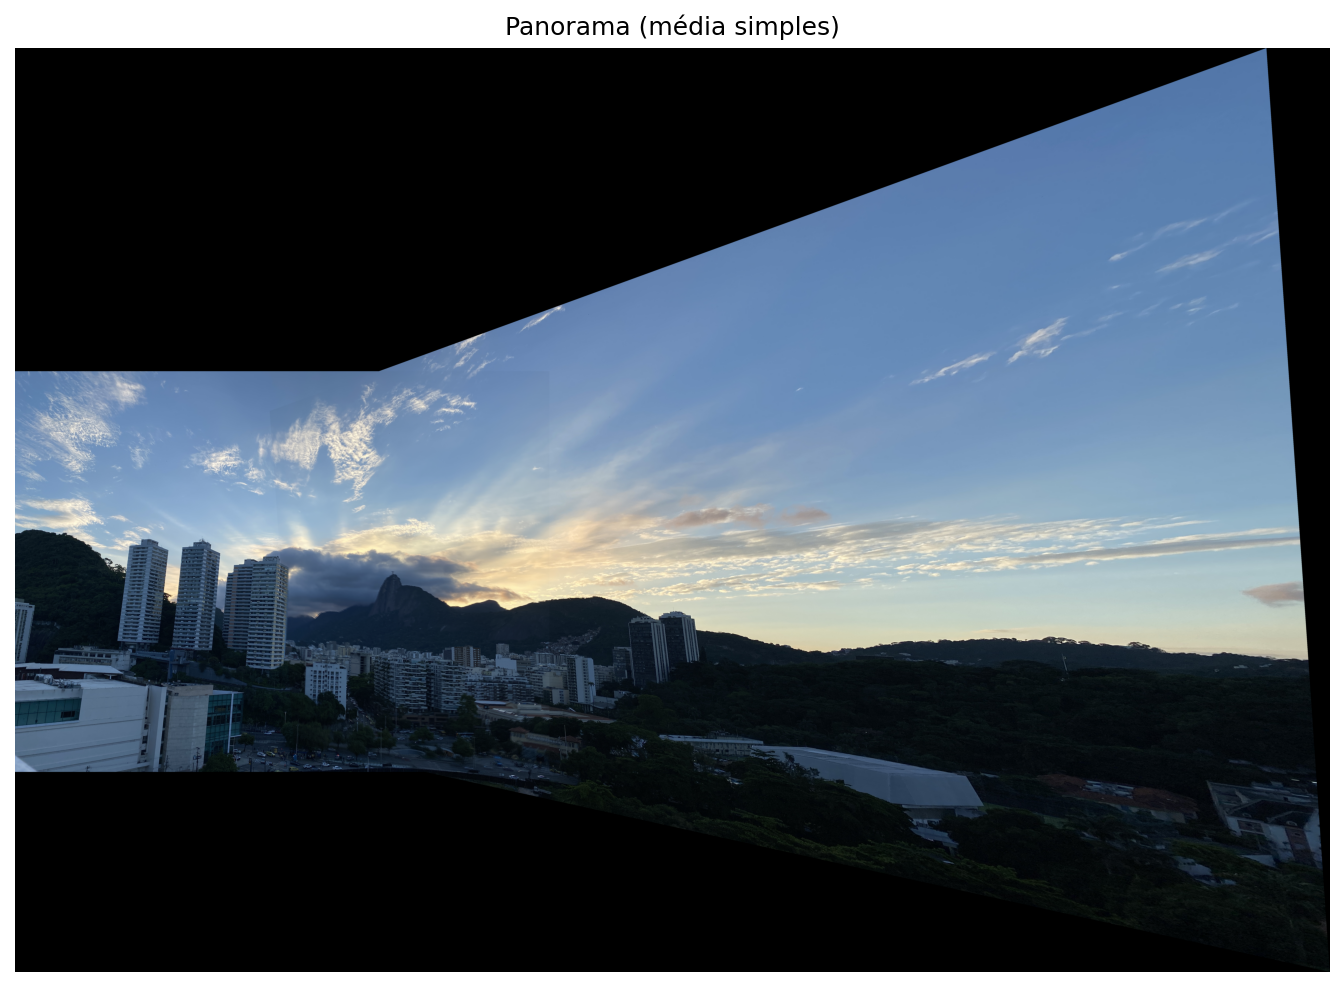
\includegraphics[width=\textwidth]{figures/ex1_panorama.png}
\caption{Panorama com média simples na sobreposição --- Exemplo 1.}
\label{fig:ex1_panorama}
\end{figure}

\subsubsection{Panorama com Blend Ponderado}

\begin{figure}[H]
\centering
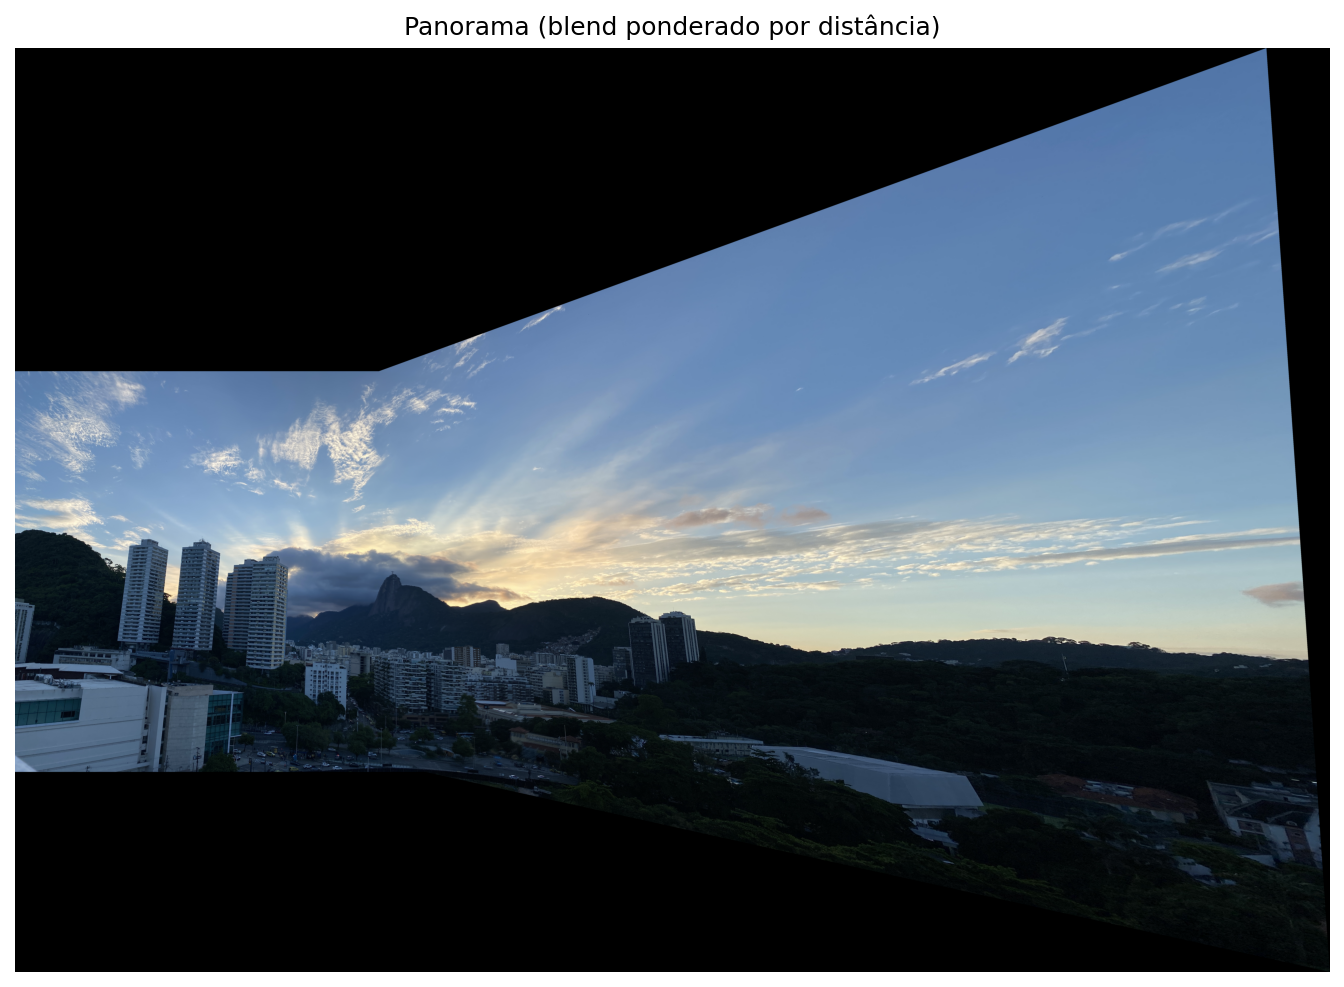
\includegraphics[width=\textwidth]{figures/ex1_blend.png}
\caption{Panorama com blend ponderado por distância --- Exemplo 1.}
\label{fig:ex1_blend}
\end{figure}

% ──────────────────────────────────────────────────
\subsection{Exemplo 2}

\subsubsection{Imagens de Entrada}

\begin{figure}[H]
\centering
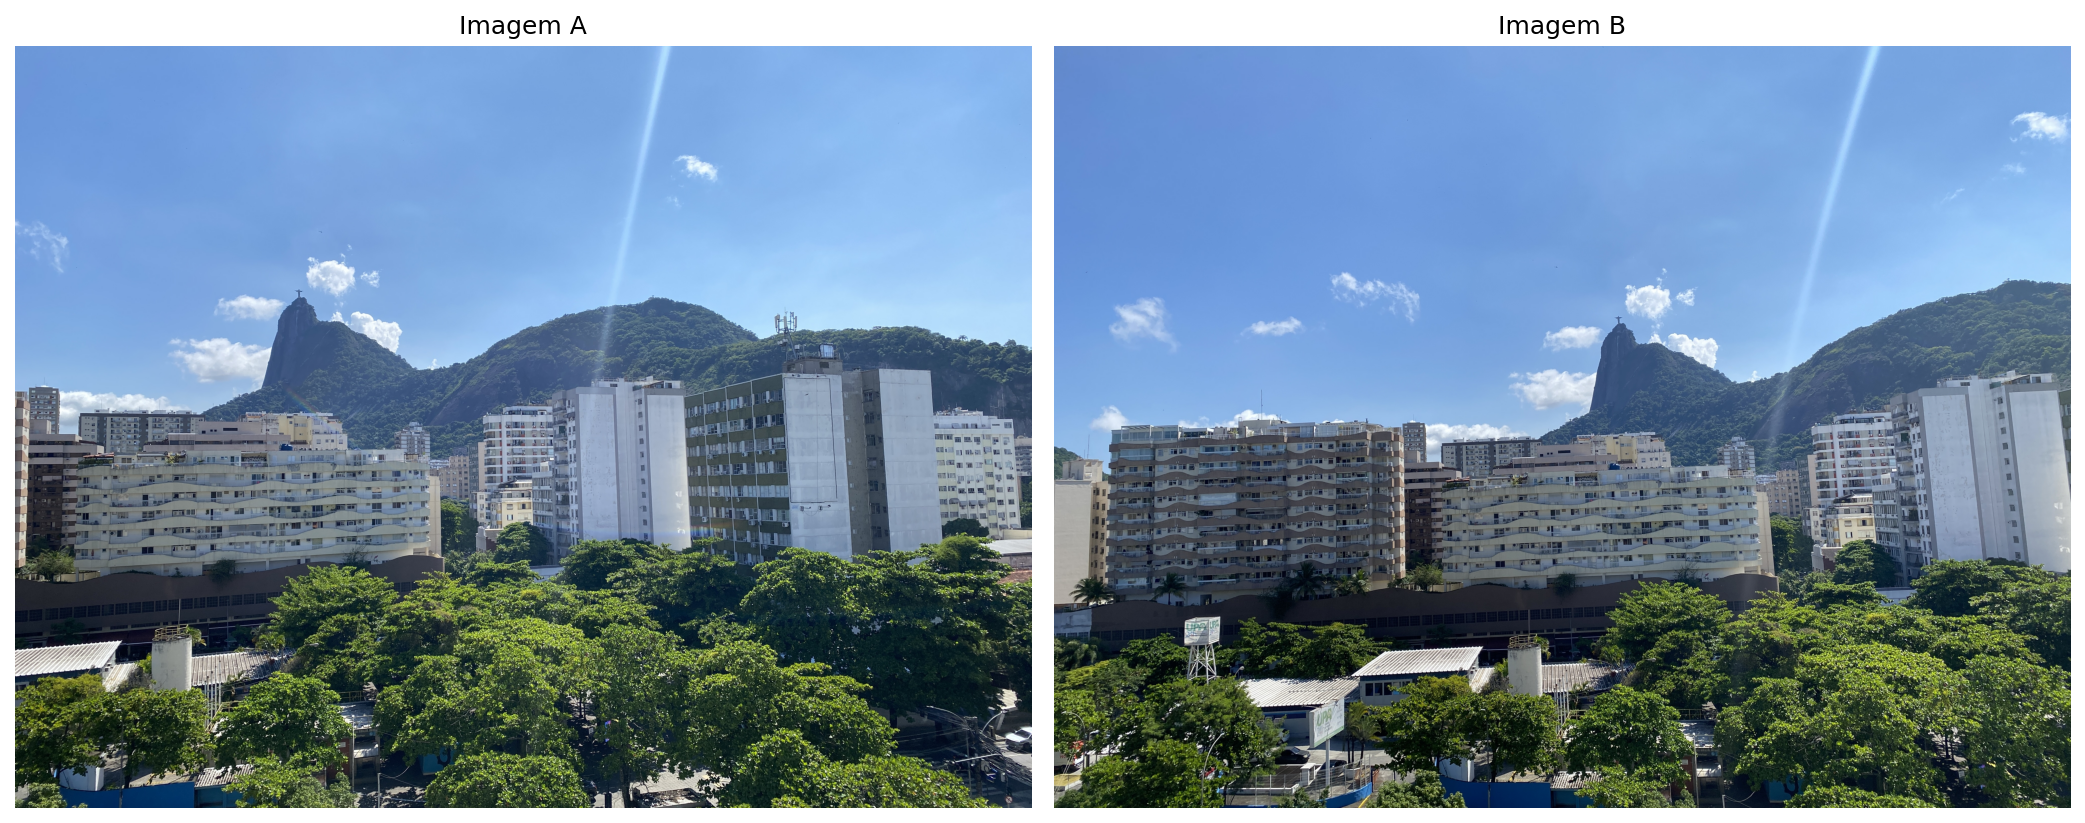
\includegraphics[width=\textwidth]{figures/ex2_inputs.png}
\caption{Imagens de entrada --- Exemplo 2.}
\label{fig:ex2_inputs}
\end{figure}

\subsubsection{Pontos Correspondentes}

\begin{figure}[H]
\centering
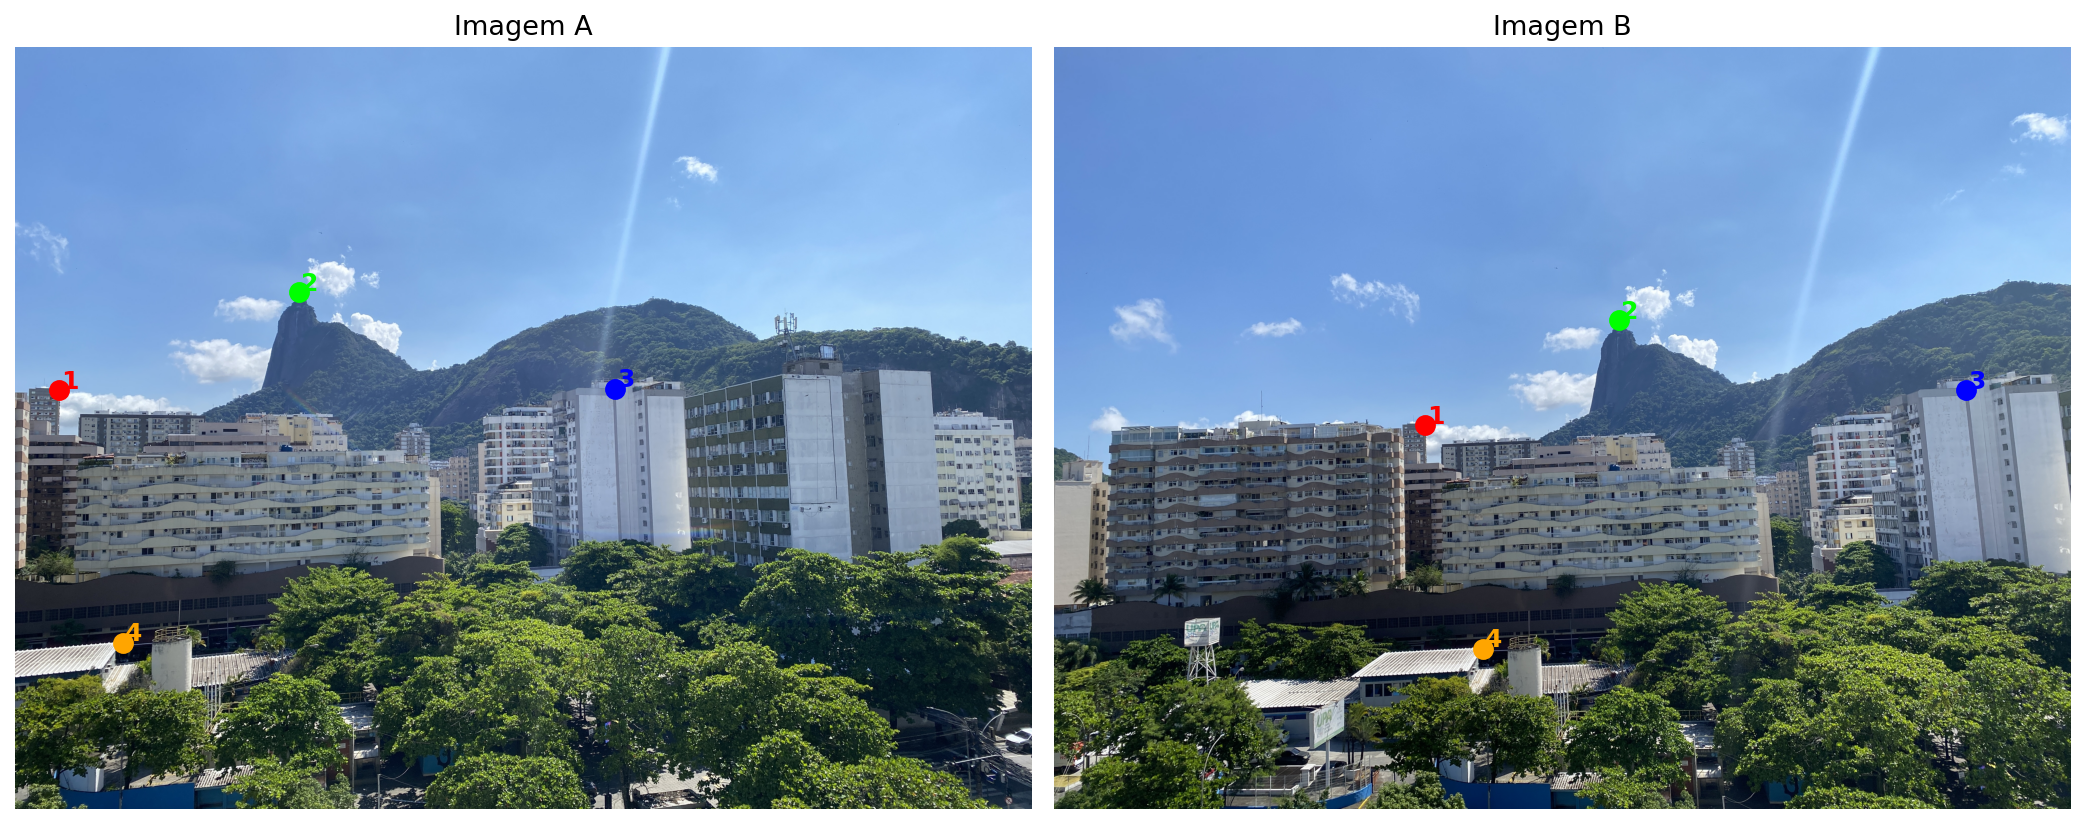
\includegraphics[width=\textwidth]{figures/ex2_points.png}
\caption{Pontos correspondentes selecionados manualmente --- Exemplo 2.}
\label{fig:ex2_points}
\end{figure}

\subsubsection{Imagem Transformada (Warped)}

\begin{figure}[H]
\centering
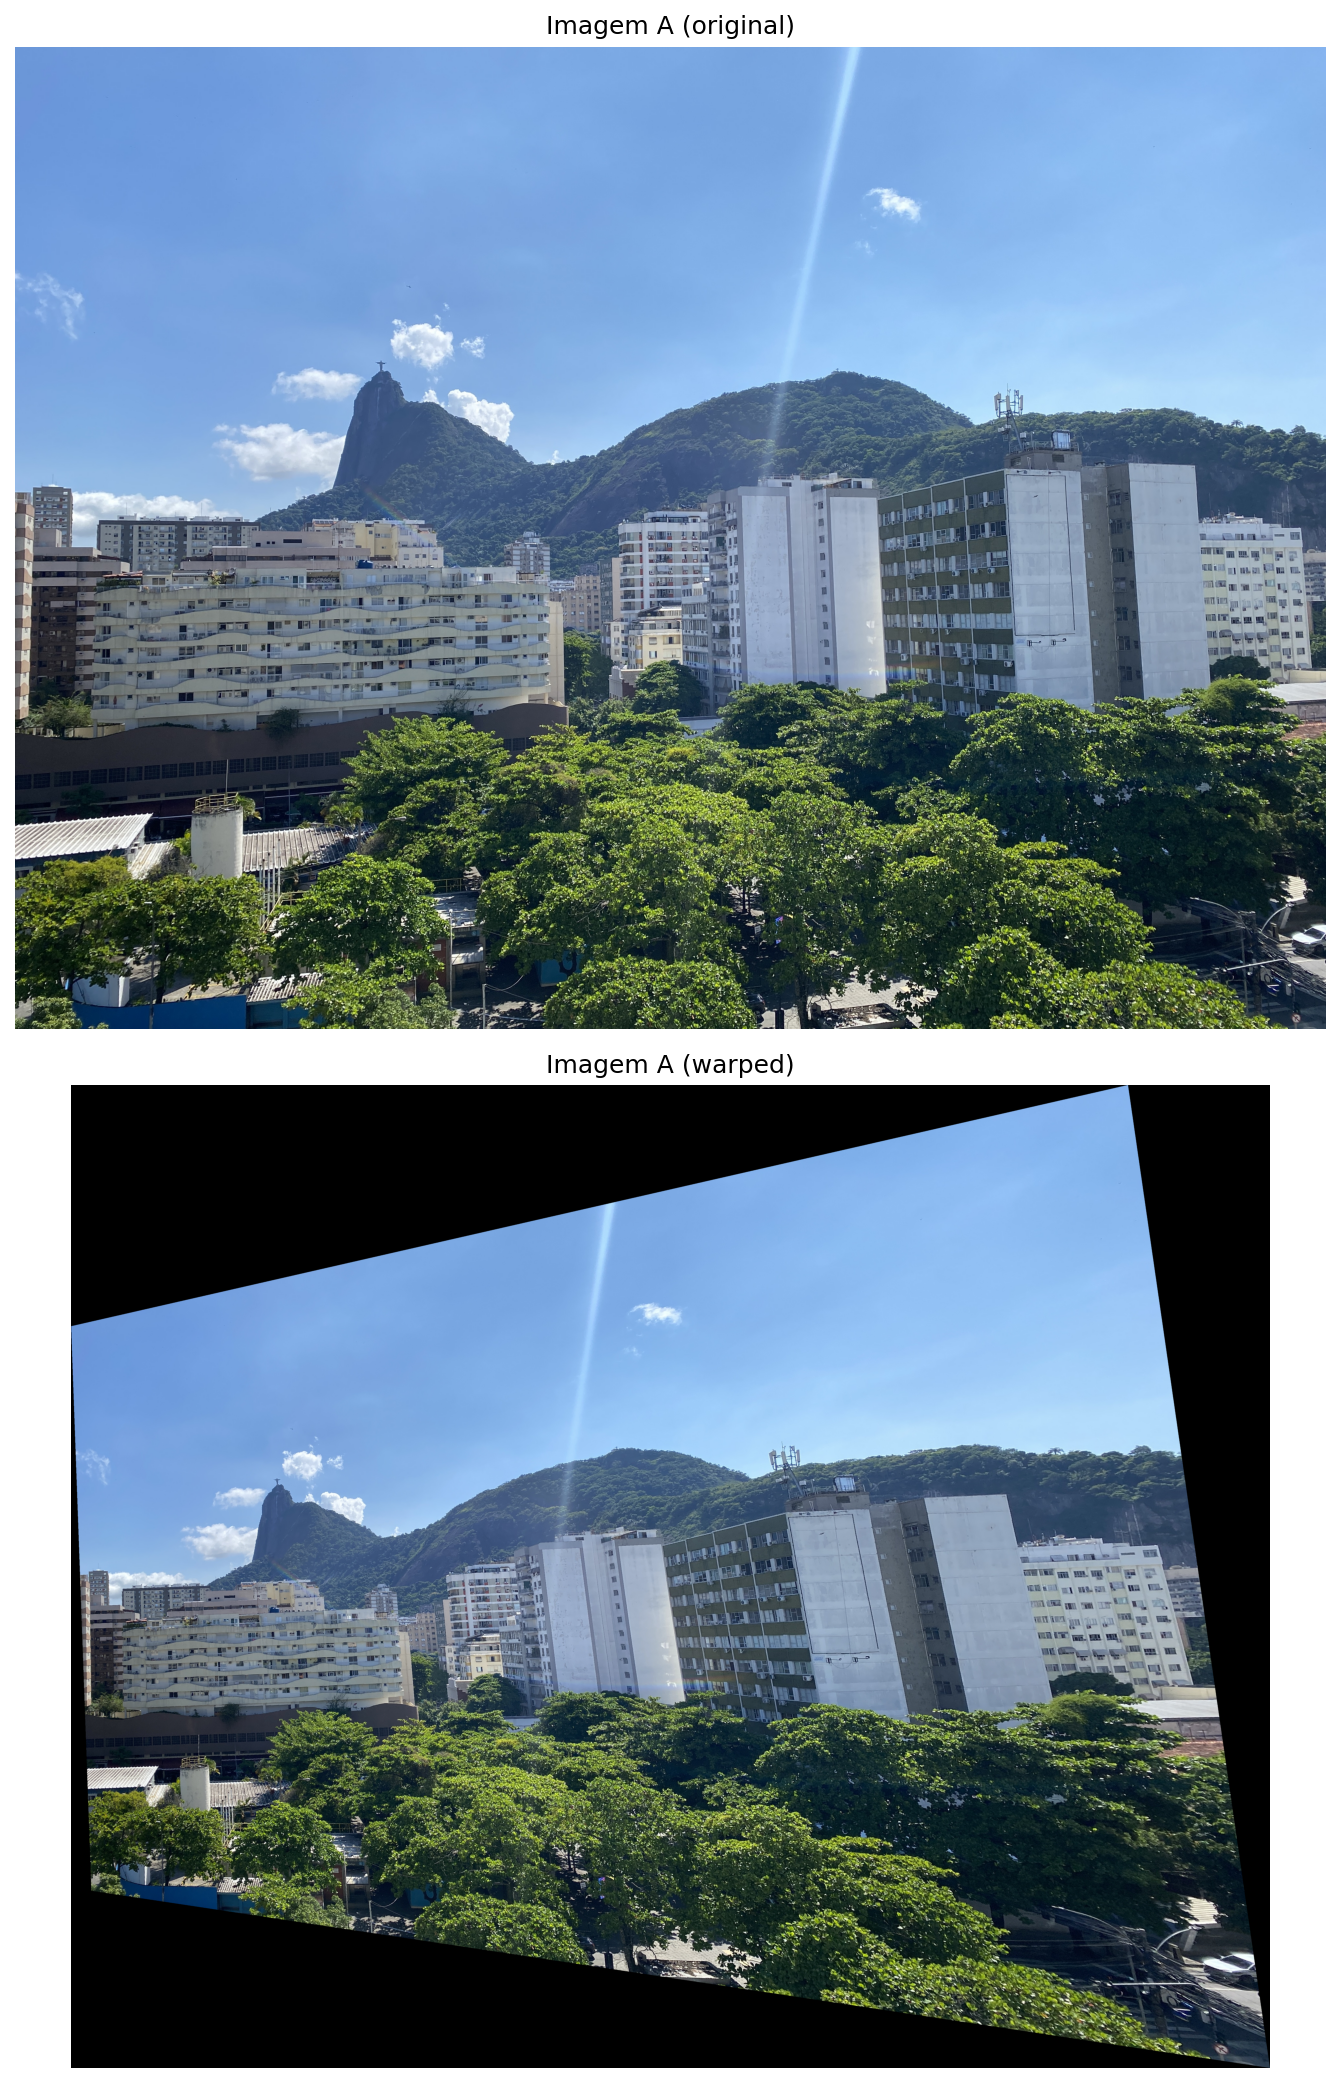
\includegraphics[width=0.85\textwidth]{figures/ex2_warped.png}
\caption{Imagem A original (acima) e após aplicação da homografia (abaixo) --- Exemplo 2.}
\label{fig:ex2_warped}
\end{figure}

\subsubsection{Panorama com Média Simples}

\begin{figure}[H]
\centering
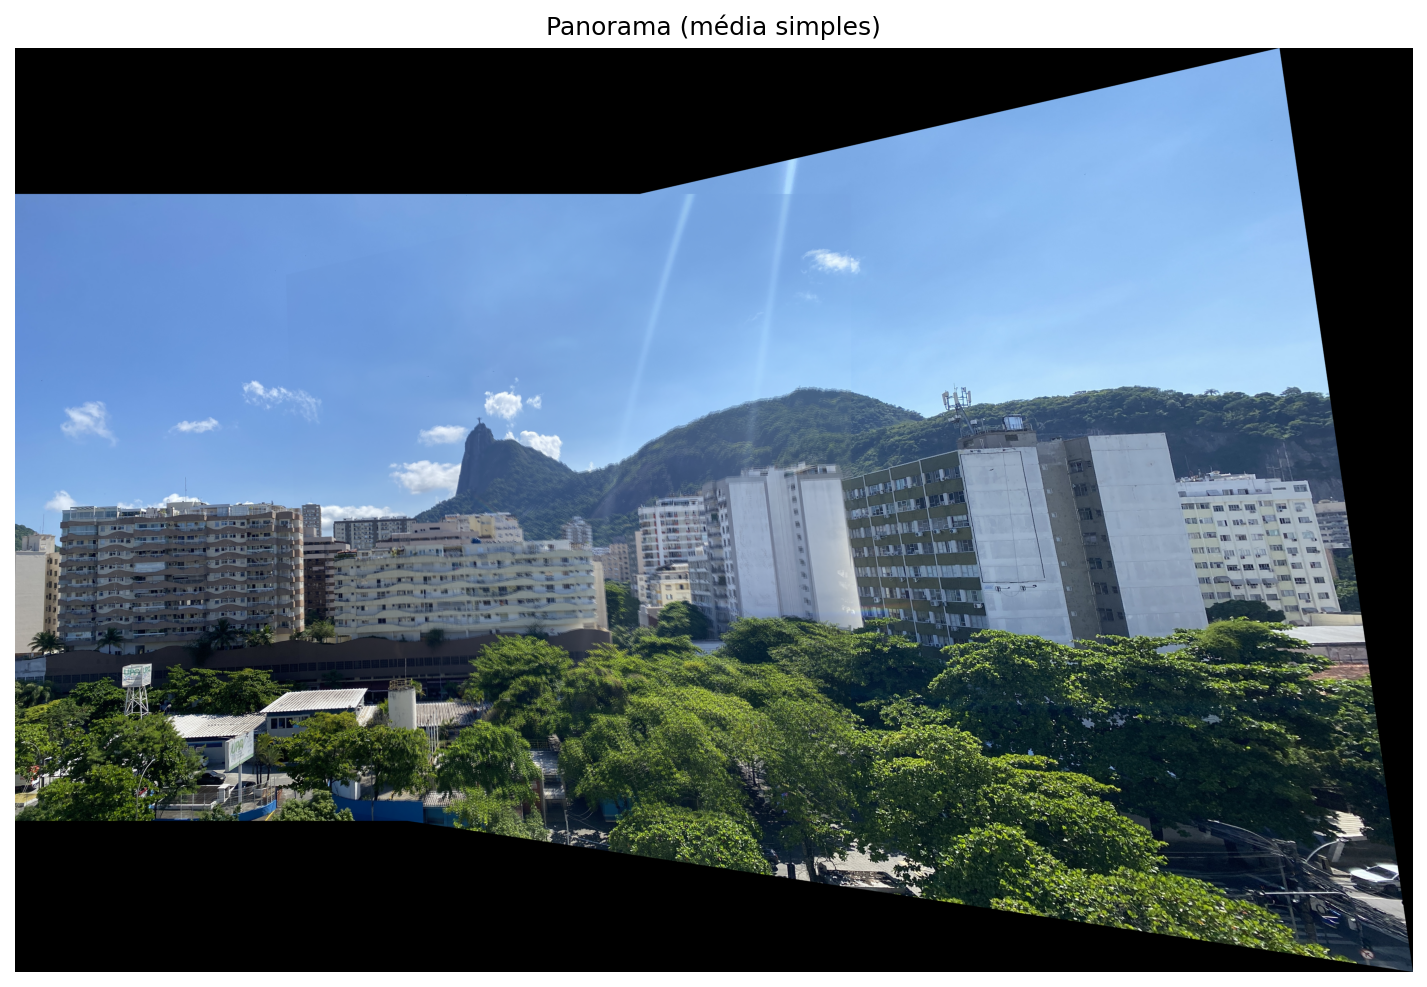
\includegraphics[width=\textwidth]{figures/ex2_panorama.png}
\caption{Panorama com média simples na sobreposição --- Exemplo 2.}
\label{fig:ex2_panorama}
\end{figure}

\subsubsection{Panorama com Blend Ponderado}

\begin{figure}[H]
\centering
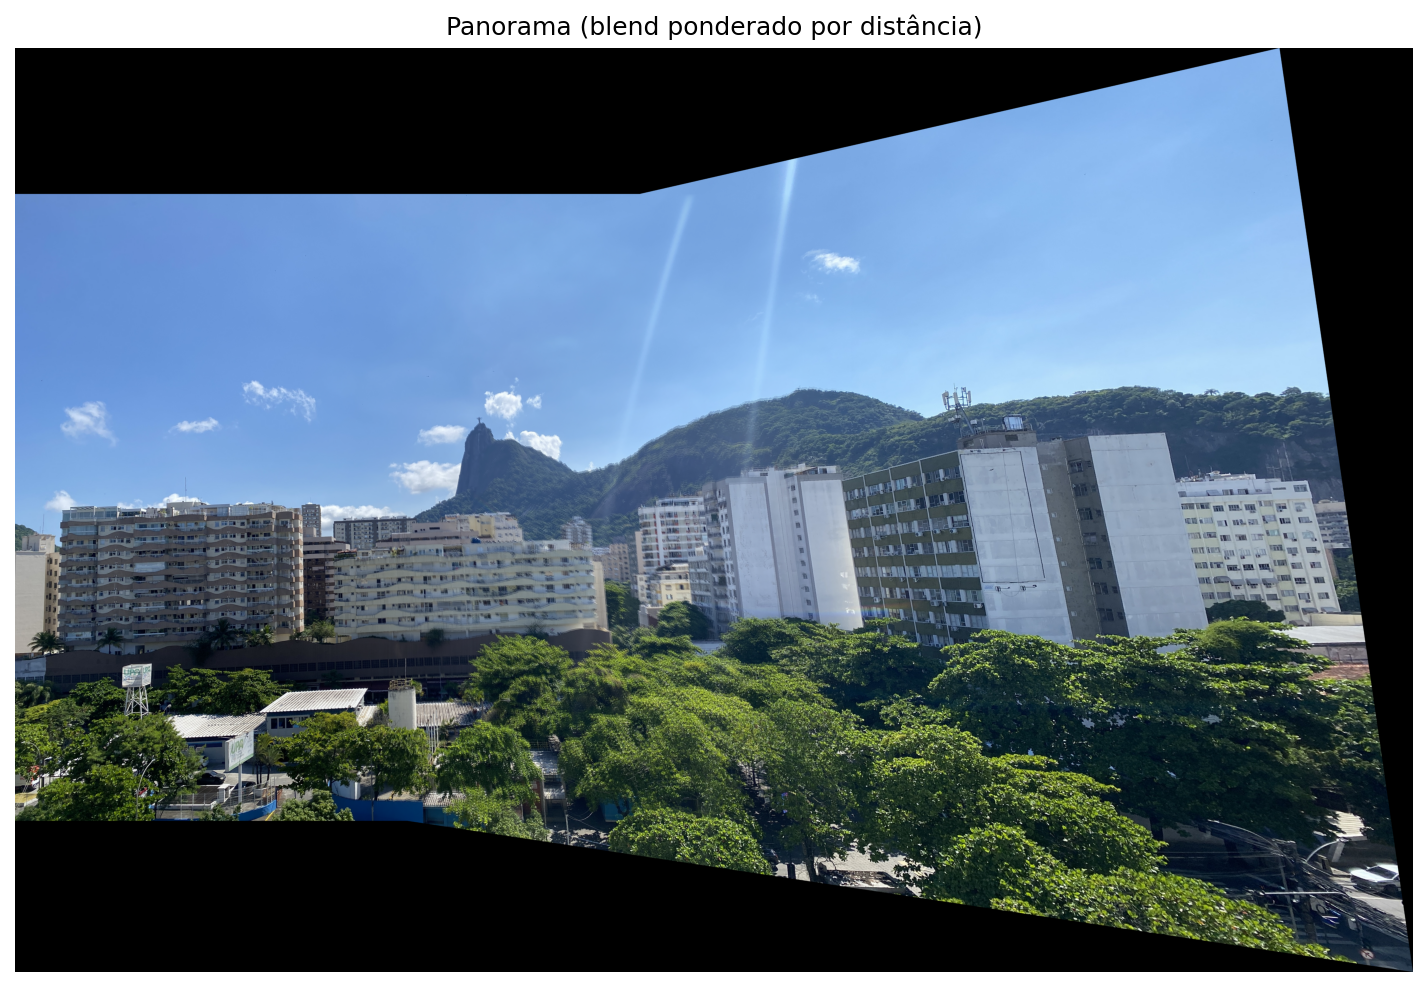
\includegraphics[width=\textwidth]{figures/ex2_blend.png}
\caption{Panorama com blend ponderado por distância --- Exemplo 2.}
\label{fig:ex2_blend}
\end{figure}

% ══════════════════════════════════════════════════════════════════════════
\section{Conclusão}

A implementação demonstrou a eficácia das transformações projetivas na Computação
Gráfica aplicada à composição de panoramas. O pipeline desenvolvido --- seleção de
correspondências, estimação da homografia via DLT/SVD, warping por mapeamento
inverso e fusão ponderada --- produziu resultados satisfatórios para os dois exemplos
testados.

O código resultante é modular, reprodutível e extensível para cenários mais
complexos, como stitching de múltiplas imagens ou adição de interpolação bilinear.

% ══════════════════════════════════════════════════════════════════════════
\newpage
\appendix
\section{Código Fonte Completo}

\subsection{Script de Seleção de Pontos (\texttt{select\_points.py})}

\lstinputlisting[caption={Script para seleção interativa de pontos correspondentes.}]
{../select_points.py}

\subsection{Notebook Principal (\texttt{photo\_stitching.ipynb}) --- Células de Código}

\begin{lstlisting}[caption={Carregamento e visualização das imagens de entrada.}]
import matplotlib.pyplot as plt
import matplotlib.image as mpimg
import os

example = 1
img_dir = f"pictures/ex_{example}"
img_files = [f for f in sorted(os.listdir(img_dir)) if str(f).endswith(".jpg")]

fig, axes = plt.subplots(len(img_files), 1, figsize=(10, 8 * len(img_files)))
if len(img_files) == 1:
    axes = [axes]

for ax, fname in zip(axes, img_files):
    img = mpimg.imread(os.path.join(img_dir, fname))
    ax.imshow(img)
    ax.set_title(fname)
    ax.axis("off")

plt.tight_layout()
plt.show()
\end{lstlisting}

\begin{lstlisting}[caption={Carregamento dos pontos correspondentes e visualização.}]
import matplotlib.pyplot as plt
import matplotlib.image as mpimg
import numpy as np
import json

COLORS = ["red", "lime", "blue", "orange"]

with open(f"{img_dir}/points.json") as f:
    data = json.load(f)

img_a = mpimg.imread(f"{img_dir}/{data['images'][0]}")
img_b = mpimg.imread(f"{img_dir}/{data['images'][1]}")
points_a = data["points_a"]
points_b = data["points_b"]

fig, (ax_a, ax_b) = plt.subplots(2, 1, figsize=(10, 16))
for ax, img, pts, label in [(ax_a, img_a, points_a, data["images"][0]),
                             (ax_b, img_b, points_b, data["images"][1])]:
    ax.imshow(img)
    ax.set_title(label, fontsize=13)
    ax.axis("off")
    for i, (x, y) in enumerate(pts):
        ax.plot(x, y, "o", color=COLORS[i], markersize=9)
        ax.text(x + 8, y - 8, str(i + 1),
                color=COLORS[i], fontsize=12, fontweight="bold")

plt.tight_layout()
plt.show()
\end{lstlisting}

\begin{lstlisting}[caption={Cálculo da homografia via DLT/SVD.}]
def compute_homography(pts_src, pts_dst):
    """
    Compute homography H such that pts_dst ~ H @ pts_src.

    pts_src, pts_dst : array-like, shape (N, 2)  N >= 4
    Returns H : ndarray, shape (3, 3), normalised so ||h|| = 1
    """
    pts_src = np.asarray(pts_src, dtype=float)
    pts_dst = np.asarray(pts_dst, dtype=float)

    rows = []
    for (x, y), (xp, yp) in zip(pts_src, pts_dst):
        rows.append([-x, -y, -1,  0,  0,  0,  xp*x,  xp*y,  xp])
        rows.append([ 0,  0,  0,  x,  y,  1, -yp*x, -yp*y, -yp])

    A = np.array(rows)
    _, _, Vt = np.linalg.svd(A)
    h = Vt[-1]
    return h.reshape(3, 3)


H = compute_homography(pts_a, pts_b)
print("H =\n", H)
\end{lstlisting}

\begin{lstlisting}[caption={Warping manual por mapeamento inverso.}]
def warp_perspective(img, M, out_size):
    """
    Warp img by the 3x3 projective matrix M via inverse mapping.

    For every pixel (x, y) in the output, we compute the corresponding
    source coordinate by applying M^{-1}, then sample with nearest-neighbour.
    Vectorised with numpy for performance.
    """
    out_w, out_h = out_size
    M_inv = np.linalg.inv(M)

    y_out, x_out = np.mgrid[0:out_h, 0:out_w]
    pixel_coords = np.stack([x_out.ravel(),
                             y_out.ravel(),
                             np.ones(out_h * out_w)])  # (3, N)

    src = M_inv @ pixel_coords                         # (3, N)

    w = src[2]
    valid_w = w != 0
    src_x = np.where(valid_w, src[0] / w, -1)
    src_y = np.where(valid_w, src[1] / w, -1)

    src_xi = np.round(src_x).astype(int)
    src_yi = np.round(src_y).astype(int)

    h_in, w_in = img.shape[:2]
    in_bounds = ((src_xi >= 0) & (src_xi < w_in)
               & (src_yi >= 0) & (src_yi < h_in))

    result = np.zeros((out_h, out_w, 3), dtype=img.dtype)
    idx = np.where(in_bounds)[0]
    result[y_out.ravel()[idx], x_out.ravel()[idx]] = \
        img[src_yi[idx], src_xi[idx]]

    return result
\end{lstlisting}

\begin{lstlisting}[caption={Cálculo da bounding box e aplicação do warping.}]
h_a, w_a = img_a.shape[:2]

corners = np.array([[0, 0], [w_a, 0], [w_a, h_a], [0, h_a]], dtype=float)
corners_h = np.c_[corners, np.ones(4)]
projected = (H @ corners_h.T).T
projected /= projected[:, 2:3]

x_min, y_min = projected[:, :2].min(axis=0).astype(int)
x_max, y_max = projected[:, :2].max(axis=0).astype(int)

out_w = x_max - x_min
out_h = y_max - y_min

T = np.array([[1, 0, -x_min],
              [0, 1, -y_min],
              [0, 0,       1]], dtype=float)

warped_a = warp_perspective(img_a, T @ H, (out_w, out_h))
\end{lstlisting}

\begin{lstlisting}[caption={Composição (stitching) com média simples.}]
h_b, w_b = img_b.shape[:2]

full_x_min = min(x_min, 0)
full_y_min = min(y_min, 0)
full_x_max = max(x_max, w_b)
full_y_max = max(y_max, h_b)

canvas_w = full_x_max - full_x_min
canvas_h = full_y_max - full_y_min

T_stitch = np.array([[1, 0, -full_x_min],
                     [0, 1, -full_y_min],
                     [0, 0,           1]], dtype=float)

warped_a_stitch = warp_perspective(img_a, T_stitch @ H,
                                   (canvas_w, canvas_h))

canvas_b = np.zeros((canvas_h, canvas_w, 3), dtype=img_b.dtype)
ox, oy = int(-full_x_min), int(-full_y_min)
canvas_b[oy:oy + h_b, ox:ox + w_b] = img_b

mask_a = warped_a_stitch.sum(axis=2) > 0
mask_b = canvas_b.sum(axis=2) > 0
overlap = mask_a & mask_b

panorama = np.zeros((canvas_h, canvas_w, 3), dtype=float)
panorama[mask_a] = warped_a_stitch[mask_a]
panorama[mask_b] = canvas_b[mask_b]
panorama[overlap] = (warped_a_stitch[overlap].astype(float)
                   + canvas_b[overlap].astype(float)) / 2
panorama = panorama.astype(np.uint8)
\end{lstlisting}

\begin{lstlisting}[caption={Máscara de distância manual para blend ponderado.}]
def get_distance_mask(img_warped):
    """
    Approximate distance-to-border weight mask (Chebyshev / L-inf).
    """
    gray = np.mean(img_warped.astype(float), axis=2)
    mask = gray > 1

    h, w = mask.shape

    h_left = np.zeros((h, w), dtype=float)
    h_left[:, 0] = mask[:, 0].astype(float)
    for x in range(1, w):
        h_left[:, x] = np.where(mask[:, x], h_left[:, x-1] + 1, 0)

    h_right = np.zeros((h, w), dtype=float)
    h_right[:, -1] = mask[:, -1].astype(float)
    for x in range(w - 2, -1, -1):
        h_right[:, x] = np.where(mask[:, x], h_right[:, x+1] + 1, 0)

    h_dist = np.minimum(h_left, h_right)

    v_top = np.zeros((h, w), dtype=float)
    v_top[0] = mask[0].astype(float)
    for y in range(1, h):
        v_top[y] = np.where(mask[y], v_top[y-1] + 1, 0)

    v_bot = np.zeros((h, w), dtype=float)
    v_bot[-1] = mask[-1].astype(float)
    for y in range(h - 2, -1, -1):
        v_bot[y] = np.where(mask[y], v_bot[y+1] + 1, 0)

    v_dist = np.minimum(v_top, v_bot)

    dist = np.minimum(h_dist, v_dist)
    max_val = dist.max()
    if max_val > 0:
        dist /= max_val
    return dist
\end{lstlisting}

\begin{lstlisting}[caption={Aplicação do blend ponderado por distância.}]
w_a = get_distance_mask(warped_a_stitch)
w_b = get_distance_mask(canvas_b)

w_a_stack = np.stack([w_a] * 3, axis=2)
w_b_stack = np.stack([w_b] * 3, axis=2)

eps = 1e-10
panorama_blend = (warped_a_stitch.astype(float) * w_a_stack +
                  canvas_b.astype(float) * w_b_stack) / \
                 (w_a_stack + w_b_stack + eps)
panorama_blend = panorama_blend.astype(np.uint8)
\end{lstlisting}

\end{document}
